\chapter{Implementación}
\label{chap:implementación}

En este capítulo se definirán las configuraciones, diagramas e implementaciones que se han llevado a cabo en el proyecto. Primero, especificaremos los diagramas de clases para el BackEnd y FrontEnd (Flujo de ejecución Django) de la aplicación.

\section{Flujo de ejecución BackEnd}

\begin{figure}[H]
  \hspace*{-.5in}{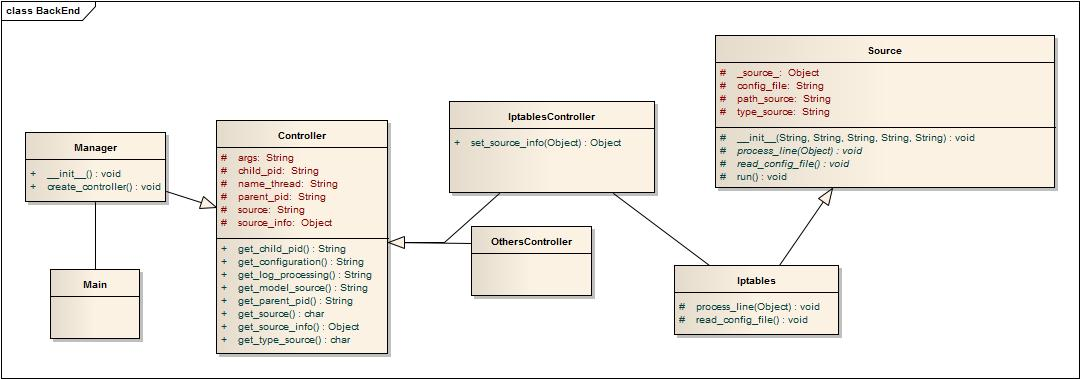
\includegraphics[scale=0.5]{diagramas/back-end.jpg}}
  \caption{Diagrama de clases BackEnd}
\end{figure}

En el diagrama podemos ver de izquierda a derecha la herencia que hay entre las clases que se encargan de recoger la información de la sonda.\\

\section{Flujo de ejecución FrontEnd}

\begin{figure}[H]
  \begin{center}
  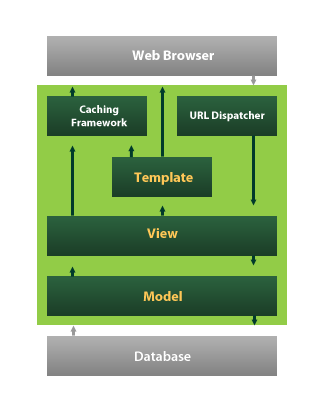
\includegraphics[scale=0.7]{diagramas/django-workflow.png}
  \caption{Flujo de ejecución del FrontEnd - ~\cite{74}}
  \end{center}
\end{figure}

Para este caso se ha decidido mostrar el flujo de ejecución que sigue una petición desde que llega al servidor de Django hasta que se sirve una vista asociada al navegador. \\

\section{Configuración de la aplicación}

En la fase de implementación del proyecto entran en juego la configuración previa de la máquina en la cuál se van a desplegar los componentes para su utilización. Hay ciertos factores a tener en cuenta. \\

Dado que se ha desarrollado una primera version funcional de la aplicación, en el futuro se podrían incluir ciertas herramientas software de automatización de despliegues y configuraciones como podrían ser:
\pagebreak
\subsection{Chef}
Web: \url{https://www.chef.io/}\\
\begin{figure}[H]
  \begin{center}
    
\includegraphics[scale=0.3]{diagramas/chef-logo.png}
  \end{center}
\end{figure}

Chef es una plataforma de automatización de gran alcance que nos transforma el control de infraestructuras en código. Da igual sobre el sistema operativo o plataforma sobre el que se tenga que operar, Chef automatiza configuraciones de infraestructuras, desplegados y gestionado a través de la red, sin importar el tamaño de la solución software a controlar.\\

A continuación un diagrama explicando la arquitectura de un sistema bajo Chef:

\begin{figure}[H]
  \begin{center}
  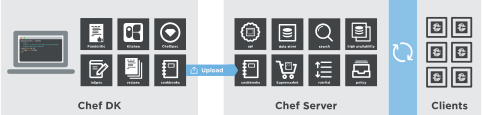
\includegraphics[scale=1]{diagramas/chef.png}
  \caption{Arquitectura de un sistema bajo Chef}
  \end{center}
\end{figure}

\subsection{Ansible}
Web: \url{https://www.ansible.com/}\\
\begin{figure}[H]
  \begin{center}
    
\includegraphics[scale=0.1]{diagramas/ansible-logo.png}
  \end{center}
\end{figure}

Ansible es una herramienta de código abierto que se utiliza para distribuir aplicaciones en nodos o servidores remotos de una manera automatizada. Nos proporciona un framework común a todas las aplicaciones, permitiendo así configurar cada una de ellas de una manera más fácil y eficaz. Ansible se basa en ``playbooks'' (al contrario de Chef que se basa en Cookbooks) dónde se pueden definir una amplia variedad de sistemas para el despliegue de una aplicación.

\begin{figure}[H]
  \begin{center}
  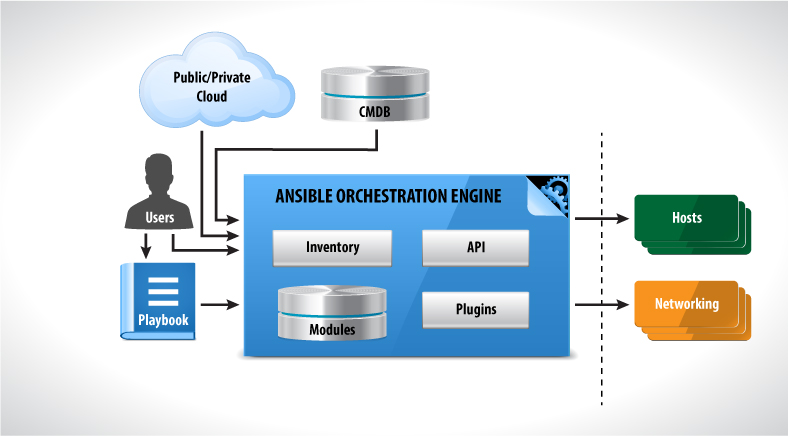
\includegraphics[scale=.5]{diagramas/ansible.jpg}
  \caption{Diagrama de la arquitectura Ansible}
  \end{center}
\end{figure}

\subsection{Docker}
Web: \url{https://www.docker.com/}\\
\begin{figure}[H]
  \begin{center}
    
\includegraphics[scale=0.5]{diagramas/docker-logo.png}
  \end{center}
\end{figure}

Docker es un sistema de desarrollo de sistemas completos, utilizando el concepto de contenedor (LXC) de los sistemas UNIX. Un contenedor de Docker, envuelve un fragmento de software en un sistema de archivos completo (imagen) que contiene todo lo necesario para funcionar: código, instancias de arranque, herramientas del sistema, bibliotecas del sistema... cualquier cosa que tendría un sistema operativo normal pero en una versión más optimizada y ligera (estos sistemas normalmente se obtienen de un Docker Repository y en su totalidad son sistemas open source). Esto garantiza que el software se ejecutará siempre de la misma forma, independientemente del medio en el que se despliegue.\\

\begin{figure}[H]
  \hspace*{-.1in}{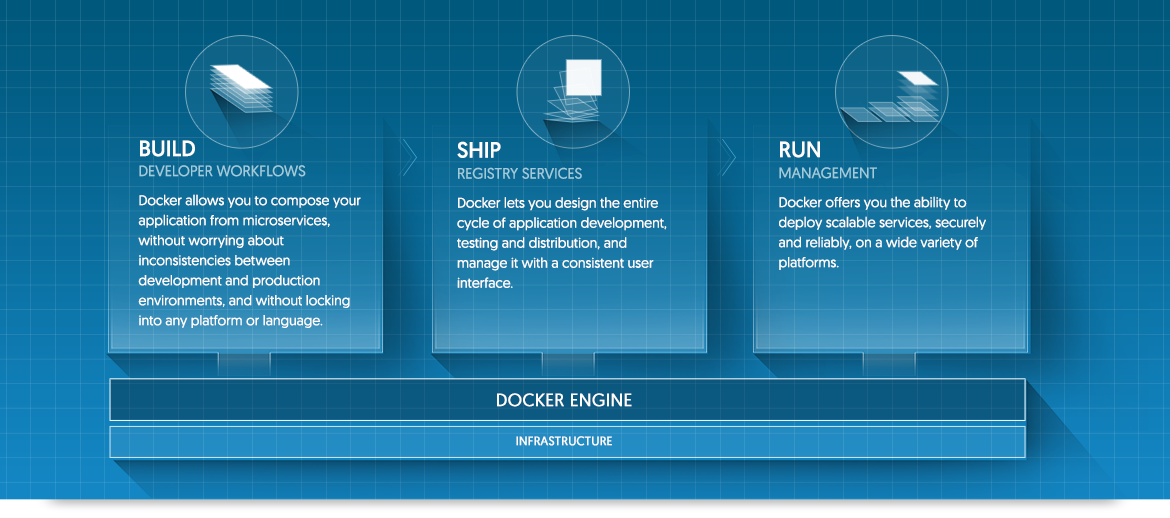
\includegraphics[scale=0.4]{diagramas/docker.png}}
  \caption{Diagrama de la arquitectura general de Docker}
\end{figure}
\newpage
\section[Configuración local]{Configuración local para procesamiento}
Los primeros pasos para la obtención de logs o eventos generados por la fuente de seguridad, iptables, serán los de configurar el sistema interno de correlación de logs rsyslog junto con el sistema de rotación de logs logrotate. Para el caso de rsyslog tenemos que definir un filtro para que cualquier evento que genere el sistema con un determinado mensaje definido en las reglas de iptables, sea capturado y almacenado en un determinado directorio. También hemos dotado a los logs del sistema de timestamp con mayor precisión para poder diferenciar eventos con mayor afinamiento y cambiado la tupla de permisos a la hora de crear un archivo con \textbf{FileCreateMode}.

\begin{figure}[H]
  \begin{lstlisting}[language=bash]
    #
    # Use traditional timestamp format.
    # To enable high precision timestamps, comment out the following line.
    #
    #$ActionFileDefaultTemplate RSYSLOG_TraditionalFileFormat

    #
    # Set the default permissions for all log files.
    #
    $FileOwner root
    $FileGroup adm
    $FileCreateMode 0644
    $DirCreateMode 0755
    $Umask 0022

    # IPTABLES

    :msg,contains,"IPTMSG= " -/var/log/iptables.log
    :msg,regex,"^\[ *[0-9]*\.[0-9]*\] IPTMSG= " -/var/log/iptables.log
    :msg,contains,"IPTMSG= " ~

  \end{lstlisting}
  \caption{Configuración de iptables para Rsyslog}
\end{figure}
\pagebreak
Hemos de configurar Logrotate (más información sobre los campos visitar sección \ref{subsection:logrotate}):

\begin{figure}[H]
\begin{lstlisting}[language=bash]
/var/log/iptables.log
        {
                rotate 7
                daily
                missingok
                notifempty
                delaycompress
                compress
                postrotate
                        invoke-rc.d rsyslog restart > /dev/null
                endscript
        }
\end{lstlisting}
\caption{Configuración de iptables para Logrotate}
\end{figure}

Tenemos que definir una regla específica para el demonio de rsyslog en la cual se filtre también por los campos que queramos de iptables:

\begin{figure}[H]
\begin{lstlisting}[language=bash]
# into separate file and stop their further processing
if  ($syslogfacility-text == 'kern') and \\
($msg contains 'IPTMSG=' and $msg contains 'IN=') \\
then    -/var/log/iptables.log
    &   ~

\end{lstlisting}
\caption{Configuración de iptables.conf para Rsyslog.d}
\end{figure}

Estos tres pasos o configuraciones nos permiten redireccionar un log de iptables al directorio \textbf{/var/log/} y en conreto para el archivo \textbf{iptables.log}. Esta configuración tendrá efecto una vez hayamos reiniciado el servico rsyslog o en el próximo inicio de sesión sobre la máquina.

\pagebreak
\subsection[Logs]{Recogida y almacenamiento de logs}
Para el caso que nos ocupa, iptables tiene una forma de definir reglas internas para el filtrado de paquetes según el tipo de comunicación que se establezca contra la máquina o desde la máquina hacia el exterior.

\begin{figure}[H]
\begin{lstlisting}[language=bash]
iptables -A INPUT -p tcp -m tcp --dport 22 -j LOG --log-prefix "IPTMSG=Connection SSH "
\end{lstlisting}
\caption{Ejemplo de regla iptables}
\end{figure}

En la siguiente sección explicaremos en profundidad cada una de las opciones de la regla, pero a simple vista podemos observar que el mensaje asociado a la regla coincide con la palabra clave del filtro empleado en rsyslog: \textbf{IPTMSG=}. Así pues, una vez dicho evento se genere el sistema y syslog lo procese como un mensaje de un servicio determinado, en este caso iptables, rsyslog filtrará dicho mensaje según su configuración para almacenarlo posteriormente en \textbf{/var/log/iptables.log}.

\subsection{Iptables}

El servicio de firewall del kernel de GNU Linux, iptables, nos proporciona una interfaz de reglas y tablas en donde podemos definir patrones o reglas que actuen sobre el tráfico que llega o sale desde nuestra máquina. Las reglas que se han definido por defecto son las siguientes (si queremos más filtros hay que implicar al protocolo y su puerto asociado con un mensaje):

\begin{figure}[H]
\begin{lstlisting}[language=bash]
# Generated by iptables-save v1.4.21 on Mon Jan 25 20:37:18 2016
*filter
:INPUT ACCEPT [0:0]
:FORWARD ACCEPT [0:0]
:OUTPUT ACCEPT [0:0]
-A INPUT -d 127.0.0.1/32 -p icmp -m icmp --icmp-type 8 -m state --state NEW,RELATED,ESTABLISHED -j LOG --log-prefix "IPTMSG=Connection ICMP "
-A INPUT -d 127.0.0.1/32 -p icmp -m icmp --icmp-type 8 -m state --state NEW,RELATED,ESTABLISHED -j DROP
-A INPUT -p tcp -m tcp --dport 22 -j LOG --log-prefix "IPTMSG=Connection SSH "
-A INPUT -p tcp -m tcp --dport 22 -j DROP
COMMIT
\end{lstlisting}
\caption{Configuración reglas iptables}
\end{figure}

A continuación una breve explicación de cada opción o comando:
\begin{itemize}
\item -A: Añadir una nueva regla a una cadena de la tabla.
\item -d: Especificación para la ip destino, en este caso localhost con una máscara de subred determinada.
\item --dport: Especificación para el puerto destino al que se realizará la posible conexión o envío de paquetes.
\item -p: Especificación del protocolo del paquete.
\item -m: Especificación de matching, en este caso icmp o tcp dentro de la descripción del paquete.
\item --icmp-type: Extensión del tipo de ping que se va a procesar desde la regla.
\item --state: Tipo de paquete según conexión:
  \begin{itemize}
  \item NEW: Paquete que crea una nueva conexión.
  \item RELATED: Paquete que está relacionado a una conexión existente, pero que no es parte de ella, como un error ICMP o, un paquete que establece una conexión de datos FTP.
  \item ESTABLISHED: Paquete que pertenece a una conexión existente (que tuvo paquetes de respuesta).
  \item INVALID (no usado): Paquete que no pudo ser identificado por alguna razón: quedarse sin memoria o errores ICMP que no corresponden a ninguna conexión conocida. Normalmente estos paquetes deben ser descartados.
  \end{itemize}
\item -j: Acción de salto cuando encuentre dicha regla de paquetes. Se especifican dos acciones:
  \begin{itemize}
  \item LOG --log-prefix ``message'' : Cuando se encuentre dicha regla se recolecta como log de la misma adjuntando un mensaje para diferenciarla del resto de reglas.
  \item DROP : Cuando se encuentre dicha regla se descarta el paquete dentro del propio sistema. Al ir seguido LOG de un DROP el paquete se muestra en el registro de syslog para posteriormente ser eliminado del registro de almacenamiento de paquetes (Para esto usamos rsyslog que se encarga de almacenar dicho mensaje en un archivo de log).
  \end{itemize}
\end{itemize}

Así pues, una vez tengamos un evento o paquete o log de iptables en nuestro sistema generados mediante ssh 127.0.0.1 o ping 127.0.0.1 obtendremos lo siguiente:

\begin{figure}[H]
\begin{lstlisting}[language=bash, breaklines=true]
[dom jul  3 17:04:03 2016] IPTMSG=Connection SSH IN=lo OUT= MAC=00:00:00:00:00:00:00:00:00:00:00:00:08:00 SRC=127.0.0.1 DST=127.0.0.1 LEN=60 TOS=0x00 PREC=0x00 TTL=64 ID=39454 DF PROTO=TCP SPT=47706 DPT=22 WINDOW=43690 RES=0x00 SYN URGP=0
[dom jul  3 17:04:05 2016] IPTMSG=Connection SSH IN=lo OUT= MAC=00:00:00:00:00:00:00:00:00:00:00:00:08:00 SRC=127.0.0.1 DST=127.0.0.1 LEN=60 TOS=0x00 PREC=0x00 TTL=64 ID=39455 DF PROTO=TCP SPT=47706 DPT=22 WINDOW=43690 RES=0x00 SYN URGP=0
\end{lstlisting}
\caption{Evento de ssh localhost en el sistema}
\end{figure}

Lo anterior correspondía a la salida del comando \textbf{\$ dmesg -T} que muestra todos los mensajes del sistema que se han pasado al syslog. La opción -T se usa para especificar el timestamp de cada mensaje con una mayor precisión.\\

\begin{figure}[H]
\begin{lstlisting}[language=bash, breaklines=true]
2016-07-03T17:03:35.664324+02:00 debian kernel: [23337.363387] IPTMSG=Connection SSH IN=lo OUT= MAC=00:00:00:00:00:00:00:00:00:00:00:00:08:00 SRC=127.0.0.1 DST=127.0.0.1 LEN=60 TOS=0x00 PREC=0x00 TTL=64 ID=39454 DF PROTO=TCP SPT=47706 DPT=22 WINDOW=43690 RES=0x00 SYN URGP=0
2016-07-03T17:03:37.668326+02:00 debian kernel: [23339.369692] IPTMSG=Connection SSH IN=lo OUT= MAC=00:00:00:00:00:00:00:00:00:00:00:00:08:00 SRC=127.0.0.1 DST=127.0.0.1 LEN=60 TOS=0x00 PREC=0x00 TTL=64 ID=39455 DF PROTO=TCP SPT=47706 DPT=22 WINDOW=43690 RES=0x00 SYN URGP=0
\end{lstlisting}
\caption{Log capturado y almacenado por rsyslog en /var/log/iptables.log}
\end{figure}

Lo anterior corresponde con la manipulación por parte de rsyslog del mensaje obtenido en syslog. Como podemos observar se añade un campo de timestamp de mayor precisión según la configuración que hemos establecido en rsyslog.conf para poder diferenciar con mayor exactitud eventos entre diferentes franjas de tiempo. \\

\begin{figure}[H]
\begin{lstlisting}[language=bash, breaklines=true]
++++++++++++++++++++++++++++++++++++++++++++++++++
--------------------------------------------------

 Procesando linea --> 2016-07-03T17:12:53.632264+02:00 debian kernel: [23896.003739] IPTMSG=Connection ICMP IN=lo OUT= MAC=00:00:00:00:00:00:00:00:00:00:00:00:08:00 SRC=127.0.0.1 DST=127.0.0.1 LEN=84 TOS=0x00 PREC=0x00 TTL=64 ID=64157 DF PROTO=ICMP TYPE=8 CODE=0 ID=14177 SEQ=7

--------------------------------------------------
++++++++++++++++++++++++++++++++++++++++++++++++++
---> Insertado registro: {'TAG': 'Connection ICMP', 'ID_Source_PORT': None, 'Protocol': u'ICMP', 'RAW_Info': '2016-07-03T17:12:53.632264+02:00 debian kernel 23896.003739 IPTMSG=Connection ICMP IN=lo OUT MAC=00:00:00:00:00:00:00:00:00:00:00:00:08:00 SRC=127.0.0.1 DST=127.0.0.1 LEN=84 TOS=0x00 PREC=0x00 TTL=64 ID=64157 DF PROTO=ICMP TYPE=8 CODE=0 ID=14177 SEQ=7 ', 'ID_Source_MAC': <Macs: 00:00:00:00:00:00:00:00:00:00:00:00:08:00>, 'ID_Source_IP': <Ips: 127.0.0.1>, 'ID_Dest_IP': <Ips: 127.0.0.1>, 'ID_Dest_PORT': None, 'ID_Dest_MAC': <Macs: 00:00:00:00:00:00:00:00:00:00:00:00:08:00>}

++++++++++++++++++++++++++++++++++++++++++++++++++
---> Fin de procesado de linea
\end{lstlisting}
\caption{Procesamiento del log capturado y almacenado en la bd interna de la aplicación}
\end{figure}
\pagebreak

\subsection[Parser]{Transformación de log en información útil: Parser}

Una vez hemos descrito los pasos a seguir para obtener un log para un evento iptables, llega la hora de procesar y hacer útil todos esos datos que tenemos. Para esta finalidad tenemos que usar expresiones regulares para generar un parser con el que ser capaz de traducir todos esos datos en información útil para nuestra aplicación.\\

\begin{figure}[H]
\lstinputlisting{trozos-codigo/codigo-4.py}
\caption{Instancia de la clase Pygtail y lectura de las líneas del log}
\end{figure}

Hacemos uso del módulo o paquete \href{https://pypi.python.org/pypi/pygtail}{Pygtail} que nos permite leer archivos de log cuyos registros internos aún no han sido leídos. Es una especie de \textbf{\$ tail -f} a un archivo en concreto, pero usa un concepto de offset e inode para saber la última actualización y posición del archivo antes y después de ser abierto para así saber que parte de la última lectura se quedo en ejecución. Éste es otro punto importante dado que para hacer uso de esta funcionalidad debemos crear un archivo con el nombre del log, véase \textbf{/var/log/iptables.log} cuya extensión final sea offset (\textbf{/var/log/iptables.log.offset}) y sus permisos los siguientes:

\begin{figure}[H]
  \begin{lstlisting}[language=bash, breaklines=true]
    -rw-r--r-- 1 root adm 10391 jul  3 17:12 /var/log/iptables.log
    -rw-r--rw- 1 root root 14 jul  3 17:13 /var/log/iptables.log.offset
  \end{lstlisting}
  \caption{Permisos de los archivos iptables.log e iptables.log.offset}
\end{figure}

Una vez tengamos el archivo abierto y con sus líneas procesadas por Pygtail, es el momento de usar regex sobre los objetos string de cada línea de log. Para ello hacemos uso del método split para dividir por palabras, es decir, posiciones separadas en una lista a todas las coincidencias con una palabra que pudiera tener toda la cadena.\\

\begin{figure}[H]
\lstinputlisting{trozos-codigo/codigo-5.py}
\caption{Uso del método split sobre la entrada de lineas de log}
\end{figure}

Una vez separado por palabras toda la línea de log, pasamos a diferenciar entre las etiquetas que iptables pone a cada campo con su valor, es decir, una tupla key=>value. \\

\begin{figure}[H]
\lstinputlisting{trozos-codigo/codigo-6.py}
\caption{Obtenemos la tupla key=>value para cada etiqueta del log}
\end{figure}

Ya tenemos todas las etiquetas de los campos del log y ahora nos toca extraer su valor asociado para asignarlo al ORM de la base de datos, es decir, almacenar la información en la BD.\\

\begin{figure}[H]
\lstinputlisting{trozos-codigo/codigo-7.py}
\caption{Vamos asignando cada etiqueta y su valor a su asociado del ORM}
\end{figure}

Los siguientes pasos de comprobación de integridad de valores y demás se relegan a la visualización del interesado en el método process\_line del archivo código fuente iptables.py\\

\pagebreak
\subsection{Workflow}
Ahora vamos a detallar los pasos que seguirá la aplicación a la hora de la visualización de información en la web mediante el framework Django. Pero primero cómo se procesan y almacenan los datos de los logs:\\

\begin{itemize}
\item Primera instancia a ejecutar main.py: Se definen las llamadas al sistema Manager que se encargará a su vez de llamar al controlador que se asocia con la fuente encargada (iptables).
\item Segunda instancia a ejecutar manager.py: Gestión de los controladores que hacen uso de la herramienta. Cada controlador tendrá asociada su fuente.
\item Tercera instancia a ejecutar controller.py: Esta clase contiene unas características que herederán los controladores de cada fuente y a su vez lanza la ejecución de los hilos para cada una de las fuentes. Aquí se define o exporta la variable de entorno de Django para utilizar el ORM del mismo.
\item Cuarta instancia a ejecutar source.py: Aunque se vaya directamente al siguiente punto, primero se pasa el control a esta clase de la cuál hereda iptables y se crean los fragmentos de código para la ejecución en iptables.
\item Quinta instancia a ejecutar iptables.py: Ejecución y configuración de todo el entramado de iptables, de la insercción de datos en la BD y de la extracción de características de los logs.
\end{itemize}

Ahora corresponde el turno al flujo de ejecución para la visualización web:\\

\begin{itemize}
\item Primera instancia a ejecutar manage.py: Aquí se cargan las configuraciones por defecto del proyecto Django para la aplicación definida.
\item Segunda instancia a ejecutar wsgi.py: Se usa la biblioteca wsgi para poder lanzar la aplicación por su nombre dentro del namespace definido por Django.
\item Tercera instancia a ejecutar settings.py: Se cargan todas las configuraciones establecidas por el usuario para el proyecto y que a su vez usarán cómo configuración base para las aplicaciones derivadas del mismo.
\item Cuarta instancia a ejecutar urls.py (archivo que pertenece al proyecto Django): Aquí se encamina la visualización entre la aplicación o la parte de administración del proyecto.
\item Quinta instancia a ejecutar urls.py (archivo que pertenece a la aplicación): Aquí es dónde se define el router de la aplicación web y los métodos que se lanzarán una vez se hagan las peticiones sobre el servidor web Django.
\item Sexta instancia a ejecutar views.py: Se ejecuta el método asociado a la renderización de la vista, que por defecto, sino hay ninguna ruta será index. Dependiendo del método a ejecutar sólo mostrará contenido estático o dinámico (JSON) obtenido de la base de datos.
\item Séptima instancia a ejecutar aplicacion/index.html (Paso previo de MasterPage.html): Se carga el trozo de esta plantilla o template (que en nuestro caso es una vista) que contiene el esqueleto principal de la parte web para todas las vistas/plantillas que heredan de esta general.
\item Octava instancia a ejecutar aplicacion/index.html (Carga de la plantilla index.html): Se carga el trozo de esta plantilla dentro del bloque definido en la plantilla MasterPage que anteriormente se proceso.
\end{itemize}


\subsection{Visualización de eventos}

Aquí tenemos una vista general de todas las interacciones posibles con la web de los eventos almacenados en el sistema.
\newpage
\begin{figure}[H]
\vspace*{.2in}{\hspace*{.55in}{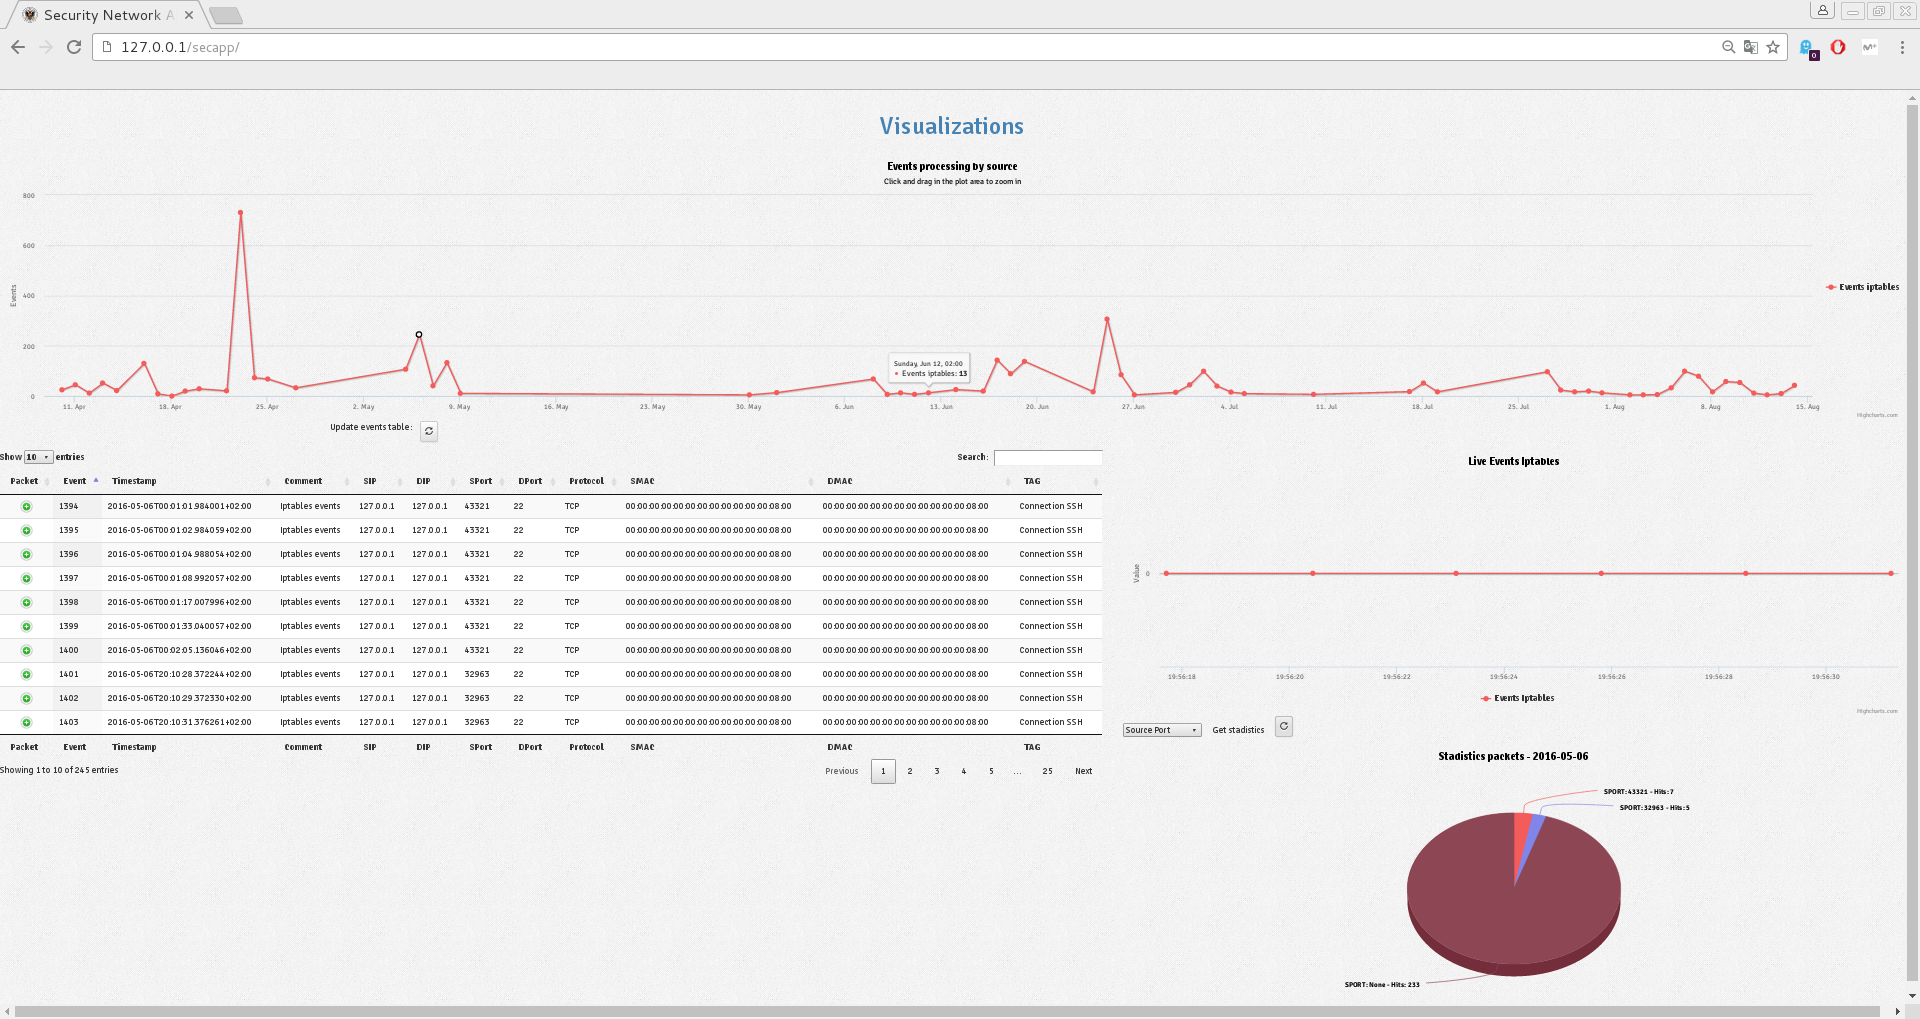
\includegraphics[scale=.33,angle=270]{diagramas/web_8.png}}}
\caption{Vista general}
\end{figure}
